\documentclass[11pt]{article}
\usepackage[top=1cm, bottom=2cm, left=1cm, right=1cm]{geometry}
\usepackage{ctex}
\usepackage{float}
\usepackage{algorithm}
\usepackage{algorithmicx}
\usepackage{algpseudocode}
\usepackage{amsthm,amsmath,amssymb}
\usepackage[colorlinks=true,linkcolor=blue]{hyperref}
\usepackage{listings}
\usepackage{xcolor,xparse}
\usepackage{realboxes}
\usepackage{graphics}
\usepackage{graphicx}
\usepackage{mathrsfs}
\usepackage{wrapfig}
\usepackage{subfigure}
\usepackage{pifont}

\definecolor{cmdbg}{rgb}{0.9,0.9,0.9}
\lstset{%
	basicstyle=\ttfamily,
	breaklines = true,
	backgroundcolor=\color{cmdbg},
}
\DeclareDocumentCommand{\ccmd}{v}{% 参数 v 表示工作方法类似于 \verb
    \Colorbox{cmdbg}{\csname lstinline\endcsname!#1!}%
}

\makeatletter
\newenvironment{breakablealgorithm}
  {% \begin{breakablealgorithm}
   \begin{center}
     \refstepcounter{algorithm}% New algorithm
     \hrule height.8pt depth0pt \kern2pt% \@fs@pre for \@fs@ruled
     \renewcommand{\caption}[2][\relax]{% Make a new \caption
       {\raggedright\textbf{\ALG@name~\thealgorithm} ##2\par}%
       \ifx\relax##1\relax % #1 is \relax
         \addcontentsline{loa}{algorithm}{\protect\numberline{\thealgorithm}##2}%
       \else % #1 is not \relax
         \addcontentsline{loa}{algorithm}{\protect\numberline{\thealgorithm}##1}%
       \fi
       \kern2pt\hrule\kern2pt
     }
  }{% \end{breakablealgorithm}
     \kern2pt\hrule\relax% \@fs@post for \@fs@ruled
   \end{center}
  }
\makeatother

\author{李明钰 22307110156}
\title{计算物理作业5}

\begin{document}
\maketitle


\section{题目1:推导二阶导数的五点公式}
\subsection{题目描述}
Derive the five-point formula for the second-order derivative.

\subsection{解答}
我们要计算函数 \( f(x) \) 在点 \( x_0 \) 的二阶导数 \( f''(x_0) \)。为此,我们考虑点 \( x_0 - 2h \),\( x_0 - h \),\( x_0 \),\( x_0 + h \) 和 \( x_0 + 2h \) 的泰勒展开:

\[
\begin{aligned}
f(x_0 - 2h) & = f(x_0) - 2hf'(x_0) + \frac{(2h)^2}{2}f''(x_0) - \frac{(2h)^3}{6}f'''(x_0) + \frac{(2h)^4}{24}f^{(4)}(x_0) - \cdots, \\
f(x_0 - h) & = f(x_0) - hf'(x_0) + \frac{h^2}{2}f''(x_0) - \frac{h^3}{6}f'''(x_0) + \frac{h^4}{24}f^{(4)}(x_0) - \cdots, \\
f(x_0 + h) & = f(x_0) + hf'(x_0) + \frac{h^2}{2}f''(x_0) + \frac{h^3}{6}f'''(x_0) + \frac{h^4}{24}f^{(4)}(x_0) + \cdots, \\
f(x_0 + 2h) & = f(x_0) + 2hf'(x_0) + \frac{(2h)^2}{2}f''(x_0) + \frac{(2h)^3}{6}f'''(x_0) + \frac{(2h)^4}{24}f^{(4)}(x_0) + \cdots.
\end{aligned}
\]

将这四个展开式加起来,注意到 \( f'(x_0) \) 和 \( f^{(3)}(x_0) \) 项会抵消:

\[
\begin{aligned}
f(x_0 - 2h) + 16f(x_0 - h) - 30f(x_0) + 16f(x_0 + h) + f(x_0 + 2h) &= 12h^2 f''(x_0) + O(h^4).
\end{aligned}
\]

我们可以从中提取 \( f''(x_0) \) 的逼近值:

\[
f''(x_0) \approx \frac{f(x_0 - 2h) - 4f(x_0 - h) + 6f(x_0) - 4f(x_0 + h) + f(x_0 + 2h)}{h^2}.
\]

这就是二阶导数的五点公式。

\subsection{伪代码}



\begin{breakablealgorithm}
    
\caption{五点法求二阶导数}
\label{五点法求二阶导数}
\begin{algorithmic}[1]
\Procedure{FivePointSecondDerivative}{$f, x_0, h$}
    \State $f_{-2} \gets f(x_0 - 2h)$
    \State $f_{-1} \gets f(x_0 - h)$
    \State $f_{0} \gets f(x_0)$
    \State $f_{1} \gets f(x_0 + h)$
    \State $f_{2} \gets f(x_0 + 2h)$
    \State $f''(x_0) \gets \frac{f_{-2} - 4f_{-1} + 6f_{0} - 4f_{1} + f_{2}}{h^2}$
    \State \Return $f''(x_0)$
\EndProcedure
\end{algorithmic}
\end{breakablealgorithm}

\section{题目2:不同的求积分方法对比}
\subsection{题目描述}
Radial wave function of the 3s orbital is: $R_{3s}(r) = \frac{1}{9\sqrt{3}} \times (6 - 6 \rho + \rho^2) \times Z^{3/2} \times e^{-\rho/2}$, where:
\begin{itemize}
    \item $r =$ radius expressed in atomic units (1 Bohr radius = 52.9 pm)
    \item $e \approx 2.71828$
    \item $Z =$ effective nuclear charge for that orbital in that atom.
    \item $\rho = \frac{2 Z r}{n}$ where $n$ is the principal quantum number (3 for the 3s orbital)
\end{itemize}

Compute $\int^{40}_{0} |R_{3s}|^2 r^2 \, dr$ for Si atom ($Z=14$) with Simpson's rule using two different radial grids:
\begin{enumerate}
    \item Equal spacing grids: $r[i] = (i-1) h; \, i = 1, \cdots, N$ (try different $N$)\label{Equal spacing grids}
    \item A nonuniform integration grid, more finely spaced at small $r$ than at large $r$: $r[i] = r_0 (e^{t[i]} - 1); \, t[i] = (i-1) h; \, i = 1, \cdots, N$ \\
    (One typically choose $r_0 = 0.0005$ a.u., try different $N$). (1 a.u. = 1 Bohr radius)\label{A nonuniform integration grid}
    \item Find out which one is more efficient, and discuss the reason.
\end{enumerate}

\subsection{程序描述}
首先,简单画出被积分函数的大致图像
\begin{equation}
    f(r) =r^2R_{3s}(r) = r^2\times \frac{1}{9\sqrt{3}} \times (6 - 6 \rho + \rho^2) \times Z^{3/2} \times e^{-\rho/2}
\end{equation}

然后根据算法\ref{不同N下的积分计算},计算出对不同N两种不同积分网格划分方式下用辛普森积分法(算法\ref{Simpson's Rule Integration}和用自适应辛普森积分法(算法\ref{Adaptive Simpson's Rule})计算出的积分结果,画出积分结果随N的变化趋势,和两种积分方法下两种网格划分的区别,最终选择用自适应辛普森积分和非均匀积分网格作为最终的计算方法。

\subsection{运行结果}
\begin{figure}[H]
    \centering
    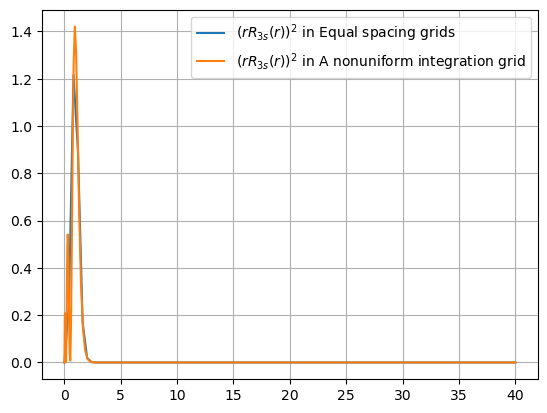
\includegraphics[width=0.5\linewidth]{被积函数图像.png}
    \caption{被积函数图像}
    \label{fig:被积函数图像}
\end{figure}

\begin{figure}[H]
    \centering
    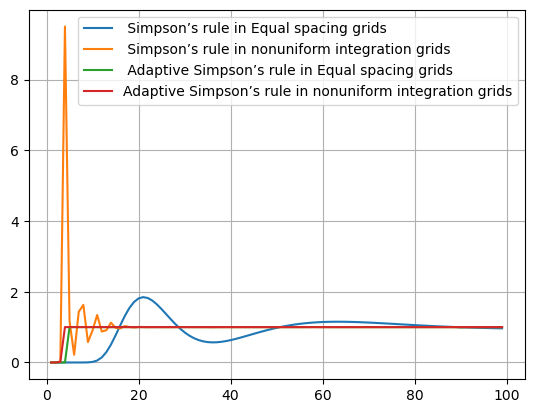
\includegraphics[width=0.5\linewidth]{不同积分方法结果.png}
    \caption{不同积分方法结果}
    \label{fig:不同积分方法结果}
\end{figure}

\begin{figure}[H]
    \centering
    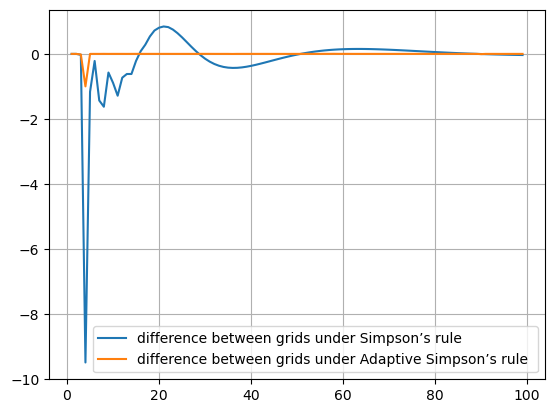
\includegraphics[width=0.5\linewidth]{两种积分规则下两种网格划分方式的区别.png}
    \caption{两种积分规则下两种网格划分方式的区别}
    \label{fig:两种积分规则下两种网格划分方式的区别}
\end{figure}

\begin{figure}[H]
    \centering
    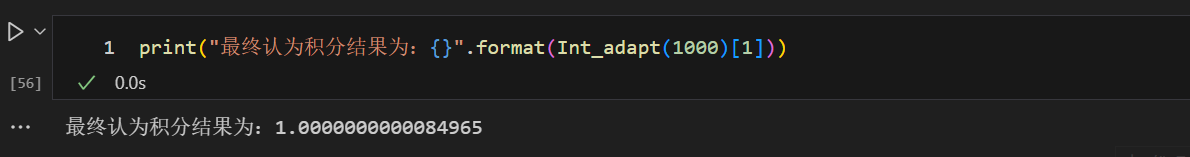
\includegraphics[width=0.5\linewidth]{最终积分结果.png}
    \caption{最终积分结果}
    \label{fig:最终积分结果}
\end{figure}

\subsection{讨论}
由被积函数图像(图\ref{fig:被积函数图像})可以看出,被积分函数在r较小时函数变化速度较快,在r较大时几乎不再变化,第二种网格划分方式\ref{A nonuniform integration grid},在r较小的部分取点较密集在r较大的部分取点较稀疏,与被积函数性质相适应,因此其误差较小,表现为图\ref{fig:不同积分方法结果}中橙色线随N增大较快收敛。

而使用自适应辛普森积分法(算法\ref{Adaptive Simpson's Rule}),则会自动在网格内找到一合适的积分区间,因此不同网格划分几乎没有差别。

\subsection{伪代码}

\begin{breakablealgorithm}

\caption{不同$N$下两种网格划分方式的积分计算}
\label{不同N下的积分计算}
\begin{algorithmic}[1]
\Procedure{ComputeIntegrals}{$r_{\text{min}}, r_{\text{max}}, N, r_0, f$}
    \State $r\_array1 \gets \text{linspace}(r_{\text{min}}, r_{\text{max}}, N)$  \Comment{创建等间距数组}

    \State $h2 \gets \frac{\ln\left(\frac{r_{\text{max}}}{r_0} + 1\right)}{N - 1}$  \Comment{计算步长因子}
    \State $t\_array \gets \text{arange}(N) \times h2$  \Comment{创建 t 数组}
    \State $r\_array2 \gets r_0 \times (\exp(t\_array) - 1)$  \Comment{创建非等间距数组}

    \State $int1 \gets 0$
    \State $int2 \gets 0$

    \For{$i \gets 0$ to $N - 2$}
        \State $int1 \gets int1 + \text{Int}(f, r\_array1[i], r\_array1[i + 1])$  \Comment{在 $r\_array1$ 上积分}
        \State $int2 \gets int2 + \text{Int}(f, r\_array2[i], r\_array2[i + 1])$  \Comment{在 $r\_array2$ 上积分}
    \EndFor

    \State \Return $int1, int2$
\EndProcedure
\end{algorithmic}
    
\end{breakablealgorithm}
\begin{breakablealgorithm}

\caption{辛普森法积分(Simpson's Rule Integration)}
\label{Simpson's Rule Integration}
\begin{algorithmic}[1]
\Procedure{SimpsonIntegration}{$f, a, b, n$}
    \State $h \gets \frac{b - a}{n}$  \Comment{计算步长}
    \State $S \gets f(a) + f(b)$  \Comment{初始化积分和}
    
    \For{$i \gets 1$ to $n - 1$}
        \If{$i$ 是奇数}
            \State $S \gets S + 4 \cdot f(a + i \cdot h)$  \Comment{奇数项系数为4}
        \Else
            \State $S \gets S + 2 \cdot f(a + i \cdot h)$  \Comment{偶数项系数为2}
        \EndIf
    \EndFor

    \State $S \gets \frac{h}{3} \cdot S$  \Comment{乘上 $\frac{h}{3}$ 得到最终积分结果}
    \State \Return $S$
\EndProcedure
\end{algorithmic}
    
\end{breakablealgorithm}


\begin{breakablealgorithm}
\caption{自适应辛普森法积分(Adaptive Simpson's Rule Integrations)}
\label{Adaptive Simpson's Rule}
\begin{algorithmic}[1]
\Procedure{AdaptiveSimpson}{$f, a, b, \epsilon$}
    \State $m \gets \frac{a + b}{2}$
    \State $S1 \gets \frac{b - a}{6} \left( f(a) + 4f(m) + f(b) \right)$  \Comment{整个区间的辛普森法估计}
    \State $S2 \gets \frac{m - a}{6} \left( f(a) + 4f\left(\frac{a + m}{2}\right) + f(m) \right)$  \Comment{左半区间的估计}
    \State $S3 \gets \frac{b - m}{6} \left( f(m) + 4f\left(\frac{m + b}{2}\right) + f(b) \right)$  \Comment{右半区间的估计}
    \State $S2 \gets S2 + S3$  \Comment{组合左半区间和右半区间的结果}

    \If {$|S2 - S1| < 15 \cdot \epsilon$}
        \State \Return $S2 + \frac{S2 - S1}{15}$  \Comment{返回积分值和误差估计}
    \Else
        \State \Return \Call{AdaptiveSimpson}{$f, a, m, \frac{\epsilon}{2}$} + \Call{AdaptiveSimpson}{$f, m, b, \frac{\epsilon}{2}$}  \Comment{递归计算}
    \EndIf
\EndProcedure
\end{algorithmic}
    
\end{breakablealgorithm}

\end{document}
